\chapter{Kademlia Network Customization and Analysis}
\label{cha:cha2}
{
Kademlia is a communication protocol for P2P overlay networks. 
It is one of many versions of a DHT, which is designed by Petar Maymounkov and David Mazières.
A Kademlia network is characterized by three constants, which were called \emph{alpha, B, and k}.
\emph{alpha} is a small number representing the degree of parallelism on network calls, usually 3.
\emph{B} is the length of keys used to identify nodes and store and retrieve data.
\emph{k} is the the number which indicates the max size of a k-bucket that contains the contacts.
Simply to say, the DHT of kademlia is different with that of Chord, CAN, Pastry and other algorithms, because Kad uses a special \emph{XOR} metric as the base of the distance calculation, which establishs an absolutely new DHT toplogy structure that advances the speed of route quering.

Kademlia itself doese not specify how to do file sharing or other network services, but defines the routing policy of communication, and four RPCs protocol functions to maintian the system which are PING, STORE,FIND\_NODE and FIND\_VALUE.
This chapter will illustrate the work mechanism of Kademlia and customization on searching and publishing which enhances the performance of KadPeer services.

}
\section{Distributed Database -- DHT}
{
P2P system usually holds a Distributed DB to publish and search entries.
Also \emph{Kademlia} maintains a distributed database, which is a Distributed method to store data. 
In the case of the needless of server, each client takes a small scope of routing table, and also takes the role of storing a fraction of data, so as to implent indexing and stroring of the whole DHT network.
The follow chart illustrates the framework of \emph{DHT}:
\begin{center}
  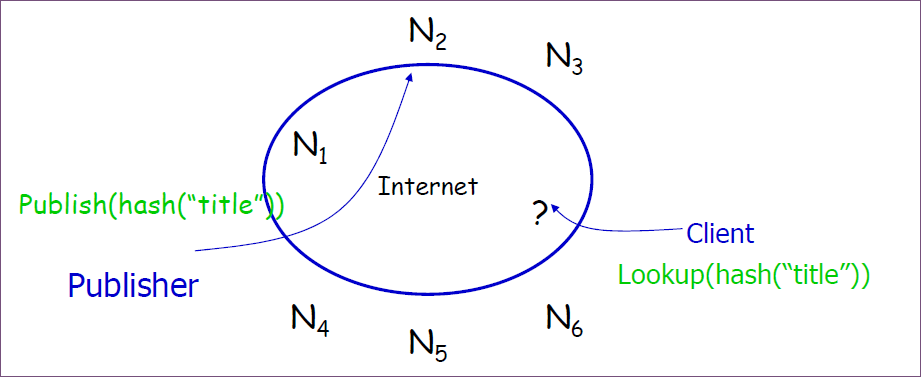
\includegraphics[width=10cm]{data/DHT.png}
\end{center}

A typical KAD DHT network may contain two dictionaries -- ``keyword dictionary'' and ``file index dictionary''.
The keyword dictionary uses the provided keyword to query the responded file name and file information. 
The key equals to the 160-bit \emph{SHA-1} hash output of the keyword; and the responded value of the key will be a list, in which lists all of the responded information of the keyword related to the file name.
Usually, these information can be presented as a triple element (file name, file length, SHA-1 value). 
The file index dictionary is used to query the file owner according to the provided file information. 
The key equals to the \emph{SHA-1} checksum of the file to be downloaded. This is because, as the aspect of statistic, the 160-bit \emph{SHA-1} checksum can ascertain a data file with specific content.
And the value to the key will be be a list as well, which contains the network information of these ndoes which might have the file.
The item of the list can be present as a triple element(IP,Port, Owner ID), by which the P2P application can query the node who has the file copy with same \emph{SHA-1} value.

}


\section{Sketch of Kademlia}
{
\emph{Kademlia} (KaD in short) is a technology of Distributed Hash Table (DHT), and the main issue of which wants to solve was information storing and indexing with distributed network-wide approach to the application layer.
In the global KaD network, all of the information were stored in the form of \textless key,value\textgreater  hash entry.
And all of the hash entry were distributed to separated nodes, and the network-wide emerged to a huge hash table. 
We can image the huge hash table to be a dictionary, that means if we get the key of index information, we can use \emph{Kademlia} protocol to locate the responded value without knowing which node the value was stored accurately.
\emph{Kademlia} takes the key role of file information indexing.
The follow chart illustrates the architecture of Kademlia protocol.
\begin{center}
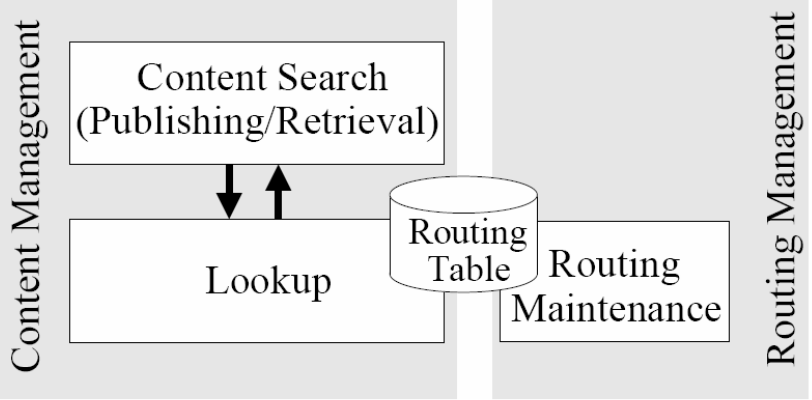
\includegraphics[width=8cm]{data/kadarchitecture.png}
\end{center}
}

\section{Components Customization of Kademlia Service}
\subsection{Routing}
\subsubsection{XOR Metric}
{
Each node in \emph{KaD} has a unique ID as identifier. 
As to the formulation of the ID, different application might have different implementation, an ordinary method was to select a unique value and do \emph{SHA-1} calculate, the unique value could be the IP of the user, or just be generated randomly.
In \emph{KadPeer} project we assume that the ID is with 160-bit length, compaired with 128-bit of the original kademlia specification.
That was because I define the length of ID is 160-bit which is the same with that of the output of \emph{SHA-1} calculation.
The distance between two nodes depends on a \emph{XOR} metric of their nodes IDs which identified the specify node.

Let node J = j$_{m}$...j$_{30}$..j$_{2}$j$_{1}$ and node K = k$_{m}$...k$_{30}$...k$_{2}$k$_{1}$, so the distance between node J and K can be calcualted as :
\begin{equation}
d(j,k) = \sum_{i=1}^{m}{
  \left\vert 
j_{i} -k_{i}
  \right\vert * 2^{i}
}
\end{equation}

we can also easily derive that the closest ID of a specific node is unique.
\begin{equation}
%\begin{align}
d(j,k) = d( j^{'},k) \Leftarrow\Rightarrow j = j^{'}
\end{equation}
\begin{equation}
d(j,k) >= 0
\end{equation}
\begin{equation}
d(j,k) = d(k,j)
\end{equation}
\begin{equation}
d(i,j) + d(j,k) >= d(i,k)
\end{equation}
\begin{equation}
d(d(i,j),d(j,k)) = d(i,k)
\end{equation}

The advantages of this \emph{XOR} metric are obvious. 
Firstly, it was easy to calculate.
Secondly, it was symmetrical which means that if node j is close to node i then node i is also close to j.
It will be useful to learn new contacts (routing table entries) just by receiving communication requests from other nodes.
}

\subsubsection{K-Bucket}
{
The routing table of Kademlia is composed by these lists which are so called k-bucket.
This is allied to \emph{Tapestry} algorithm whoes routing table is constructed similarly with that of kademlia.
Each node will store some information of these contacts with which the distance between them is in the scope [ 2$^{i-1}$,2$^{i}$) ( 0 \textless= i \textless= 160).
In the other implementation of kademlia , these information of contacts that stored in a node is composed by list of Node ID, IP and UDP port.
However in \emph{KadPeer} , it was much more complex, because I added the function of tunnel through NAT and firewalls based on the \emph{UDT} library.
I reserved the fileds of rendezvous ip and port for additional usage.
Each list of the information is so-called \emph{K-Bucket}, and the contacts in the bucket is sorted by the last visit time.
The last-recently contact is in the list head, and the most-recently is in the head tail.
Each bucket has its max size of contacts which is characterized by variable \emph{K}.
Usually, K is an even number which is used to balance the system performance and the network load.
The chart below illustrates the structure of a K-Bucket.
\begin{center}
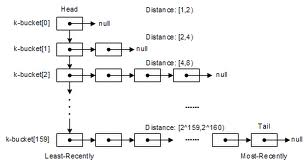
\includegraphics[width=8cm]{data/kbucket.jpg}
\end{center}

When variable ``i'' is very small, the K-Bucket will be empty; while the variable increasing, the items in the bucket will exceed K.
It is because the growth of the discance that the K-Bucket covered is exponential, that means a node will know more the closer neighbors and less farther ones which ensures the convergence of the information query process.
That is to say, every node knows well of its neighbors and as the distance growth the degree will decline.
As the interval is divided by exponentially, so the complexity of key looking up of a N nodes kad network is log(N).
This feature is simliar with that of \emph{Chord} fingertable of interval spiliting.
When a node i receives a RPC message , the sender node contact info of j in i node's k-bucket will be updated.
The steps are as followed:
\begin{enumerate}\itemsep1pt
\item Calculate the distance between iteself and the sender node : d(i,j).
\item Select responded K-Bucket to do update according to the calculated distance d.
\item If contact of j is on the selected bucket, then move the contact to end of the bucket.
\item If contact of j is not on the selected bucket
\begin{enumerate}%[I]%
\item If the size of the selected bucket is smaller than k, then add the contact information of node j to the end of the bucket.
\item If the size of the selected bucket is greater than k, then select the head contact z in the bucket to do Ping RPC.
\begin{enumerate}%[(a)]%
\item If the z node doese not send the response message, then delete the contact of z and add contact of j to the end of the bucket.
\item If the z node sends the response message, the move contack of z to the end of the bucket and drop j.
\end{enumerate}
\end{enumerate}
\end{enumerate}

The mechanism of bucket update method implements the strategy of updating last-see node, unless the on line nodes have never been removed from the bucket.
That is to say, the longer the node on the line, the more it will be leaved on the K-Bucket.
With this mechanism, KaD can obviously improve the online rate of the contacts in the bucket.
This will bring up greate advantages on the stabilty of kad network and decline of maintenance cost.
On the other hand, this mechanism can defend \emph{DDos} attacking, as only when the old nodes are out of ervice, these new nodes can be joined into the k-bucket, which avoids the flooding of the routing information caused by joining of the new peers.
In order to prevent the K-Bucket from getting old, the KaD will select some node from the k-bucket it contains to do RPC\_PING during the interval that there is no k-bucked updated.
The mentioned updateing mechanism of KaD moderates the bottleneck of the traffic, all of the nodes will not do the updating operation at the same time.
At the same time, KaD can respond the nodes which are out of service rapidly.
}

\subsubsection{Routing Table Evolution}
{
When Node u wants to joion the KaD network, it should communicate with an existed node w.
First of all, u adds contact of w to its own K-Bucket, then send a RPC\_FIND\_NODE.
After that, u will update its K-Bucket according to the information that has gethered.
By quering the neighbors from far to near by steps, node finished the construction of the empty routing table, and publish the contact of its own to the neighbors.
In KaD, the routing table of each node is present as a binary tree, and the leaf can be considered as a K-Bucket.
We take node as an example, the process of routing table construction is as followed:
\begin{enumerate}
\item At first, routing table in node u is a simple K-Bucket, which covered 160-bit ID space.
\item When u learned some new node information, it will try to add these information to the responded K-Buckets:
\begin{enumerate}
\item If the K-Bucket is not full, then the new node will inject into the K-Bucket.
\item If the K-Bucket is full:
\begin{enumerate}
\item If the current bucket scope covered the ID of node u, then the current bucket would be splited as two bucket with the same size. And reassgin the contacts in each new bucket according to the prefix value.
\item If the current bucket scope does not cover the ID of node u, then the contact of u will be dropped.
\item Repeat the process listed above, and at last the routing table will be constructed which contains much contacts that are near by and less contacts that are far away.
\end{enumerate}
\end{enumerate}
\end{enumerate}
The chart below illustrates the process of K-Bucket splitting.
\begin{center}
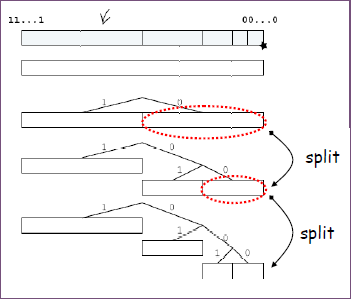
\includegraphics[width=8cm]{data/TableSplit.png}
\end{center}

}

\subsection{Searching}

\subsubsection{Iterative Quering}
{
There are two types of data quering methods. 
First is iterative quering , the second is Recursive quering.
KaD uses iterative routing for quering.
In the process of iterative quering, the source send look-up request the next hop and wait for its reply, and then according the content of the reply to query the next hop till the iteration depths reached the max value or the source has got the reqeusted data.
However ,in the process of Recursion quering, the source send look-up request the next hop but do not wait for the reply of that hop.
The second hop queries its own database to check if it has the data that the source requested.
If the hop contains the data that reqeuested, it will send the response to the source or query the next hop depending on the routing table it has till the recursion depth reached the max value.
The follow chart illustrates the core differences between iterative quering and recursive quering.
\begin{center}
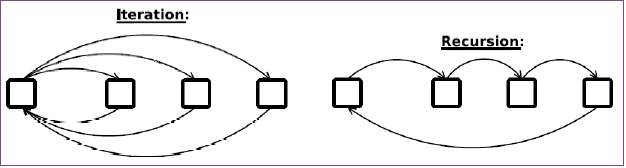
\includegraphics[width=8cm]{data/IterativeLookup.png}
\end{center}

Considering with the process of iterative quering, the source is responsible for the whole process, and at each step, source send requests and wait for the reply,
so the advantages of iterative quering are much easier to observe:
Firstly, Lookup messages cannot be lost due to the departure of an intermediate peer holding the lookup request.
Secondly, Iterative routing is easier to debug since information at each step is reported back to source.
}



\subsubsection{Parallel Look-Up}
{
In Kademlia algorithm, in ordor to reduce the problem of hitting stale contacts and improves lookup performance, it takes parallel mechanism to do data look up, although this will inevitably brings up the traffic of quering process.
Source simultaneously issues multiple lookup requests to different peers and continues the lookup process based on the information obtained from all requests.

The follow chart illustrates the process of parallel look-up.
\begin{center}
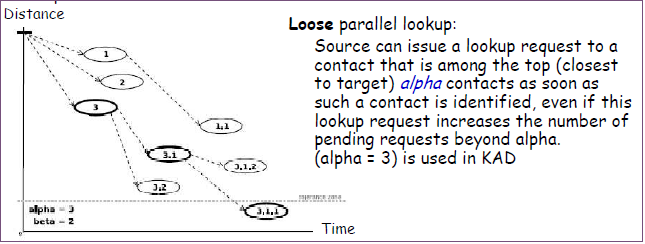
\includegraphics[width=15cm]{data/ParallelLookup.png}
\end{center}

%Source can issue a lookup request to a contact that is among the top (closest to target) alpha contacts as soon as such a contact is identified, even if this lookup request increases the number of pending requests beyond alpha. (alpha = 3) is used in KAD.
}

\subsubsection{Kad Node Status}
{
In \emph{Kademlia} network, all of the nodes can be considered as a leaf of a binary tree, and the location of a node was decided by the shortest prefix of the ID.

For any node can separate the binary tree into series of continuous, non-self-contained subtrees.
The top level subtree was composed of the whole tree excludes the subree of its own, and the next layer subtree was composed of the rest half subtree;and so forth, till the whole tree was separated. The next chart illustrates how to separate a tree by node ``0011''.
\begin{center}
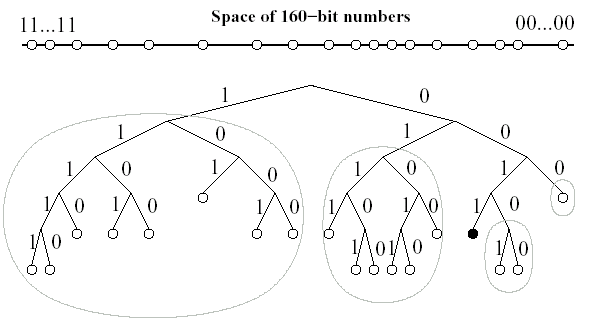
\includegraphics[width=10cm]{data/kadbintree.png}
\end{center}

The parts which were contained by dotted line were respective subtrees. the prefix from top to the bottom were `1','01' ,'000' ,'0010'.
\emph{KaD} protocol makes sure that each node knows at least one node of the subtrees, as long as these subtrees are not null.
In this context, each node can find the other nodes by the unique ID.
The process of routing was obtained through the efforts of the distance of \emph{XOR}.
The chart below illustrates the way that how does node ``0011'' find the node ``1110'' by continuously quering.
The node ``0011'' accesses closer to the ultimate target node convergently by progressive learning and inquiry among the bottom of the sub-trees.
Should be noted that, the only node ``101'' was known by node ``0011'' . 
\begin{center}
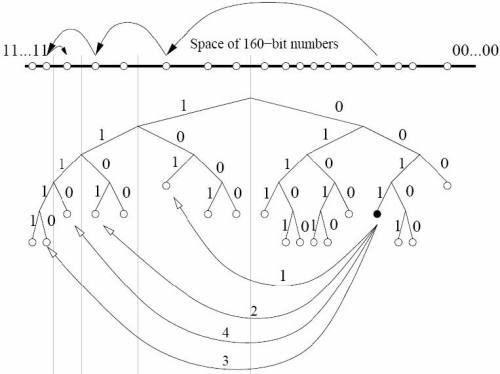
\includegraphics[width=8cm]{data/kademlialookup.jpg}
\end{center}
Should be noted that, the only node ``101'' was known by node ``0011'' 
}

\subsubsection{Optional Choking}
{
In Kademlia, there is no definition of the policy on contact choosing while the RPC FIND\_VALUE reply of quering contains multiple contacts.
A FIND\_VALUE RPC includes a B=160-bit key. If a corresponding value is present on the recipient, the associated data is returned. Otherwise the RPC is equivalent to a FIND\_NODE and a set of k triples is returned.
However, In the project of \emph{KadPeer}, I defined a policy on contacts choking based on a third party project with the name of \emph{GeoIP} which may improve the performance of P2P network services.

GeoIP is the proprietary technology that drives MaxMind's IP geolocation data and services. GeoIP provides businesses with a non-invasive way to determine geographical and other information about their Internet visitors in real-time. 
When a person visits the website, GeoIP can determine which country, region, city, postal code, and area code the visitor is coming from. 
Furthermore, GeoIP can provide information such as longitude/latitude, connection speed, ISP, company name, domain name, and whether the IP address is an anonymous proxy or satellite provider.

As the feature provided by \emph{GeoIP}, in the reply of RPC quering, the \emph{KadPeer} will get the reail time information of the contacts by calling the GeoIP API.
It will sort the contacts by the connection speed and choose these contacts which are with high connection speed for data downloading and uploading.

}

\subsubsection{Node Searching and Locating}
{
The supreme feature of Kademlia algorithm is the mechanism of quickly node searching, and the steerable quering process by changing the key parameters such as \emph{alpha} and \emph{k}.
We assume node x want to find the node whos ID is y,  kad will do as followed process to locate node y.
\begin{enumerate}
\item calcute the distance between x and y, d = d(x,y).
\item Select $\alpha$ nodes from the [log(d)$_{th}$] K-bucket of node x, and send FIND\_NODE RPC to the $\alpha$ nodes. If the the number of contacts in the K-BUCKET is less than $\alpha$, then select the enough contacts from the buckets which are closer to d.
\item As to the contacts on the reply, if the current node is y, then send the reply to the source that it is the closest node to y. Otherwise, cacluate the distance to y, and select $\alpha$ contacts from responded K-BUCKET to send to x.
\item x will send FIND\_NODE RPC to the received contacts in the reply, and redo the process till that there is node which replys the nearest ID to y in each branch. These nodes which are not quickly responded will exclude from the candidate list till they send the reply.
\item Through the operation listed above, node x will get k contacts which are closer to node y. 
Because node y might not be in the internet, we say the closer here.  $\alpha$ is the parameter which controls the parallel degree. When $\alpha$ = 1 , the searching process will be simliar with \emph{Chord} quering hops.
\end{enumerate}

Because source can get information from the bucket which is closer to destination during the query each time, this mechanism ensures that the distance to the target will be halved or at least decline one bit.
So, the efficiency of Kademlia algorithm will be log(N), and N indicates the number of nodes in the kad network.
When node x wants to search \textless key,value\textgreater, the operation is similar to search a node.
Node x will choose k contacts which are closer to key, and send FIND\_VALUE RPC to them. Then redo the process to the contacts which are contained in the replys.
When RPC FIND\_VALUE succeed, the \textless key,value\textgreater will be stored in the node which is the closest to key, so as that it will enhance the performance of quering next time.
By this way, the scope of hot \textless key,value\textgreater will be expanded,which makes the acknowledgement of whole system become more shorter.
}

\subsection{Publishing}
{
In Kademlia specification, there is no definition of how and where to publish data that users might be interested. But, it defines the interval to republish and expire which ensures that the data in the system is fresh.
However, publish process is another important performance indicator of P2P system.
}

\subsubsection{Where to Publish}
{
Where to publish a given key kID?
Unfortunately, the original \emph{Kademlia} does not define the method to the publish.
I have referred the way that how does \emph{Chard} and \emph{Emue} to publish the given data.
In \emph{Chord}, the given data will be stored in the first node with which the ID is larger than the kID.
However, in the implementation of \emph{emue}, there is a concept with the name of zone, in which the first 8 bits of the nodes are the same.
8 bits is the 1/256 of the entire key space( The key space of emue is 128 B), which contains several thousand of peers.  
In my project \emph{KadPeer}, I also followed the conception of zone.
However, I define the zone in which the first 16 bit of the nodes are the same, as the key space of kadpeer is 160-bit.
And when publishing, 16 nodes which are in the same zone with the KID are choosen for uploading the data.
That means 16 copies of publishing data will exist in the network, and this number will grow depending on how hot this data is as the time elapsing.
That is because while searching the hot key, when the source finds the key, it will send RPC STORE\_VALUE to the closest contact in its bucket to store the hot key and value pair.

However, how to find these nodes in a 16-bit zone?
To get the 16-bit zone, the source will send RPC FIND\_NODE with the parameter KID, this will obtain an ordered (by closeness) list of nodes that are up the KID.
After that, the source will send RPC PUBLISH\_REQUEST to the closer candidate nodes.
In each nodes, there will be a specify data store with multiple index and a mark field, which indicates the wether the data is published or just a common data.
In kadpeer, in order to obtain a high performance of data storing and searching in a node, I did not use  database sucha as mysql as the data store.
I implemented a data structure which can reorder the content with two indexes.
Any data published in the network will be stored in the computer memory, which ensures that the data will keep fresh cooperation with the republish policy of the kademlia algorithm.

\subsubsection{How to Publish}
Another important issue is how to publish the data.
Compared with the other P2P application, in kadpeer network there is only two kinds of data.
One is metadata of a media stream, the other one is stream data.
While publishing, the splitting engine will split the OGG stream data to pieces, and meanwhile the metadata will be generated, which contains the file name and important OGG stream information.
So, when we publish a media stream, we need to publish two components of an entry.
I defined a two-level publishing steps here.
Level 1 indicates the hash value of metadata information.
Level 2 indicates the hash media content data which has been splitted into pieces by the OGG codec engine.

We assume that a client wants to share a media file with the name of ``kademlia project''.
\begin{center}
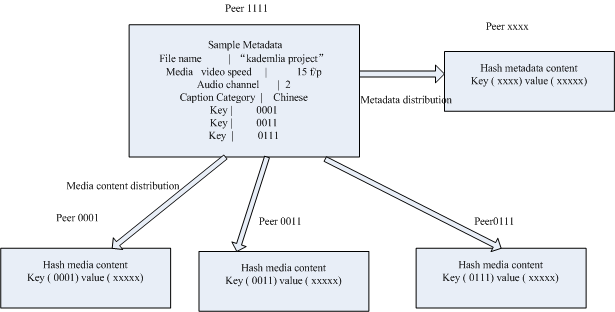
\includegraphics[width=15cm]{data/Distribution.png}
\end{center}
The OGG codec firstly parse the media file, and generate the metadata according to the content of the media, which contains the hash value of each media stream pieces.
%The ``kademlia project'' was divided in to several pieces, which content hash value was ``0011'' 
Each hash value will be the KID which covered the global kadpeer ID space.
The publisher will then distribute each hash key and value pair of the media to the 16-bit zone which covered with the key ID.
It is because that the metadata is the only identifier of a specify stream.
We need to publish it to the network so as to the other peer can find it as well.

%\begin{center}
%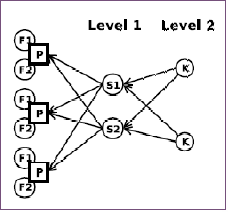
\includegraphics[width=5cm]{data/TwoLevel.png}
%\end{center}

}

\section{Summary}
{
%This chapter, I have illustrated the way that the \emph{Kademlia} network worked, and also interpreted the customization on the algorithm.
The latest work of P2P is incarnateed on the decentralised structured network toplogy basd on DHT.
The essence of DHT is a huge hash table which is maintained by a profusion of nodes in union.
The DHT is splitted into pieces, and each node will maintain a chunck of table which belongs to it.
The nodes of DHT is dynamic and also is generous,so decentralised-structured and self-ruled are the importand target of design.
An object or a keyword can be hashed to a 128 or 160 bit space by calculating the hash function.

DHT liked structure is self-adapting for node join and leave, and with good performance, expandability, vigorousness, and the ablity of self-organization.
It is because that the overlay network adapt to confirmative structure, the DHT can support accurate discovery.
As soon the node is on the network as it could be found.
This chapter will illustrate the work mechanism of Kademlia and customization, which provides network modes for VoD on demond system.

}

